\begin{figure}
    \centering
    \begin{minipage}[b]{0.36\linewidth}
    \begin{subfigure}{\linewidth}
        \centering
        \begin{tikzpicture}[hypergraph,xscale=1.2,yscale=1.2]
            \node[vertex,label={east:$x_1$}] (x1) at (0, 0) {};
            \node[vertex,label={south:$x_2$}] (x2) at (0, -1) {};
            \node[vertex,label={north:$x_3$}] (x3) at (0, 1) {};
            \node[vertex,label={north:$x_4$}] (x4) at (-1, 0) {};
            \node[vertex,label={east:$x_5$}] (x5) at (1, 0) {};

            \node[vertex,label={south:$x_6$}] (x6) at (0, -2) {};
            \node[vertex,label={north:$x_7$}] (x7) at (0, 2) {};
            \node[vertex,label={north:$x_8$}] (x8) at (-1, 1) {};
            \node[vertex,label={east:$x_9$}] (x9) at (-2, 0) {};
        
            \begin{scope}[on background layer]
                
                \newcommand*{\pathri}{($(x1) + (0,0.5)$)
                    to[out=0,in=0] ($(x6) + (0,-0.5)$)
                    to[out=180,in=180] ($(x1) + (0,0.5)$)
                }
                    
                \newcommand*{\pathrii}{($(x7) + (0,0.6)$)
                    to[out=0,in=90] ($(x7) + (0.5,0)$)
                    to[out=-90,in=90] ($(x2) + (0.5,0)$)
                    to[out=-90,in=0] ($(x2) + (0,-0.6)$)
                    to[out=180,in=-90] ($(x2) + (-0.5,0)$)
                    to[out=90,in=-90] ($(x7) + (-0.5,0)$)
                    to[out=90,in=180] ($(x7) + (0,0.6)$)
                }
                
                \newcommand*{\pathriii}{($(x1) + (0.3,-0.3)$)
                    to[out=45,in=-45] ($(x3) + (0.3,0.3)$)
                    to[out=135,in=45] ($(x8) + (-0.3,0.3)$)
                    to[out=-135,in=135] ($(x4) + (-0.3,-0.3)$)
                    to[out=-45,in=-135] ($(x1) + (0.3,-0.3)$)
                }

                \newcommand*{\pathriv}{($(x9) + (-0.25,0)$)
                    to[out=90,in=90] ($(x1) + (0.5,0)$)
                    to[out=-90,in=-90] ($(x9) + (-0.25,0)$)
                }

                \newcommand*{\pathrv}{($(x1) + (-0.25,0)$)
                    to[out=90,in=90] ($(x5) + (0.5,0)$)
                    to[out=-90,in=-90] ($(x1) + (-0.25,0)$)
                }
                
                \draw[hyperedge,looseness=1,draw=Red,fill=Red,fill opacity=.1] \pathri;
                \draw[hyperedge,looseness=1,draw=Fuchsia,fill=Fuchsia,fill opacity=.1] \pathrii;
                \draw[hyperedge,looseness=1,draw=Gray,fill=Gray,fill opacity=.1] \pathriii;
                \draw[hyperedge,looseness=1, draw=BurntOrange,fill=BurntOrange,fill opacity=.1] \pathriv;
                \draw[hyperedge,looseness=1, draw=Cyan,fill=Cyan,fill opacity=.1] \pathrv;
        
                \node[text=Red] at (-0.9,-2) {$R_1$};
                \node[text=Fuchsia] at (-0.6,2.5) {$R_2$};
                \node[text=Gray] at (-1.4,1.5) {$R_3$};
                \node[text=BurntOrange] at (-2,-0.75) {$R_4$};
                \node[text=Cyan] at (1.3,-0.6) {$R_5$};
                
            \end{scope}
        \end{tikzpicture}
        \caption{Hypergraph}
        \label{fig:complicated-hg}
    \end{subfigure}
    \end{minipage}
    \hfill
    \begin{minipage}[b]{.63\linewidth}
    \begin{subfigure}{\linewidth}
        \centering
        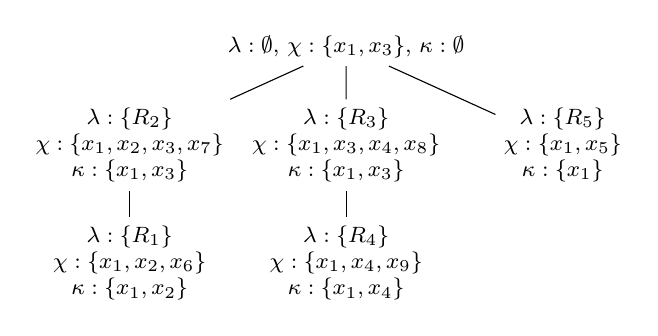
\begin{tikzpicture}[
			level 1/.style={level distance=1.25cm, sibling distance=2.75cm},
            level 2/.style={level distance=1.5cm, sibling distance=1.4cm},
            xscale=1,yscale=1
        ]
        \footnotesize
			\node { $\lambda: \emptyset$, $\chi: \{ x_1, x_3 \}$, $\kappa: \emptyset$ }
				child { node[align=center] {$\lambda: \{R_2\}$ \\ $\chi: \{ x_1, x_2, x_3, x_7 \}$ \\ $\kappa: \{ x_1, x_3 \}$} edge from parent[-]
                    child { node[align=center] {$\lambda: \{ R_1 \}$ \\ $\chi: \{ x_1, x_2, x_6 \}$ \\ $\kappa: \{ x_1, x_2 \}$} edge from parent[-] }
                }
                child { node[align=center] {$\lambda: \{ R_3 \}$ \\ $\chi: \{ x_1, x_3, x_4, x_8 \}$ \\ $\kappa : \{ x_1, x_3 \}$} edge from parent[-]
                        child { node[align=center] {$\lambda: \{ R_4 \}$ \\ $\chi: \{ x_1, x_4, x_9 \}$ \\ $\kappa: \{ x_1, x_4 \}$} edge from parent[-] }
                }
                    child { node[align=center] {$\lambda: \{ R_5 \}$ \\ $\chi: \{ x_1, x_5 \}$ \\ $\kappa : \{ x_1 \}$} edge from parent[-] }
                ;
		\end{tikzpicture}
        \vspace{-0.25\baselineskip}
        \caption{Meta-decomposition}
        \label{fig:complicated-meta}
    \end{subfigure}
    
    \vspace{0.5\baselineskip}
    
    \begin{subfigure}{.32\linewidth}
        \centering
        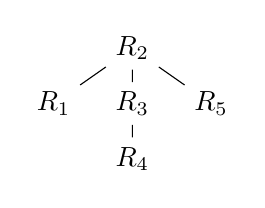
\begin{tikzpicture}[
			level distance=0.7cm,
			level 1/.style={sibling distance=1cm}
        ]
			\node { $R_2$ }
				child { node {$R_1$} edge from parent[-] }
                child { node {$R_3$} edge from parent[-]
                    child { node {$R_4$} edge from parent[-] }
                }
                child { node {$R_5$} edge from parent[-] } ;
		\end{tikzpicture}
        \vspace{-0.25\baselineskip}
        \caption{A join tree}
        \label{fig:complicated-jt1}
    \end{subfigure}
    \hfill
    \begin{subfigure}{.32\linewidth}
        \centering
        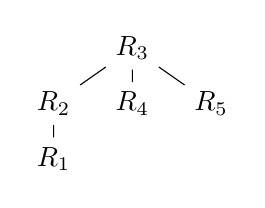
\begin{tikzpicture}[
			level distance=0.7cm,
			level 1/.style={sibling distance=1cm}
        ]
			\node { $R_3$ }
                child { node {$R_2$} edge from parent[-]
                    child { node {$R_1$} edge from parent[-] }
                }
				child { node {$R_4$} edge from parent[-] }
                child { node {$R_5$} edge from parent[-] } ;
		\end{tikzpicture}
        \vspace{-0.25\baselineskip}
        \caption{A second join tree}
        \label{fig:complicated-jt2}
    \end{subfigure}
    \hfill
    \begin{subfigure}{.32\linewidth}
        \centering
        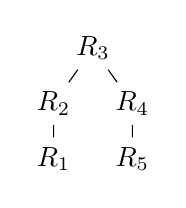
\begin{tikzpicture}[
			level distance=0.7cm,
			level 1/.style={sibling distance=1cm}
        ]
			\node { $R_3$ }
                child { node {$R_2$} edge from parent[-]
                    child { node {$R_1$} edge from parent[-]
                    }
                }
				child { node {$R_4$} edge from parent[-]
                    child { node {$R_5$} edge from parent[-] }
                };
		\end{tikzpicture}
        \vspace{-0.25\baselineskip}
        \caption{A third join tree}
        \label{fig:complicated-jt3}
    \end{subfigure}
    \end{minipage}
    \caption{Hypergraph, meta-decomposition, and three join trees of the query $Q_{\ref{ex:meta-complicated}}$ in \cref{ex:meta-complicated}}
    \label{fig:complicated}
\end{figure}

